
Les signaux originaux sont en stéréo, il faut les moyenner pour retrouver le cadre du cours et ainsi avoir des signaux en mono.
fig.\ref{Fig.sub.1} représente le signal original et fig.\ref{Fig.sub.2} représente le signal moyenné.
\begin{figure}[htb]
\subfigure[Exemple de signal audio original]{
\label{Fig.sub.1}
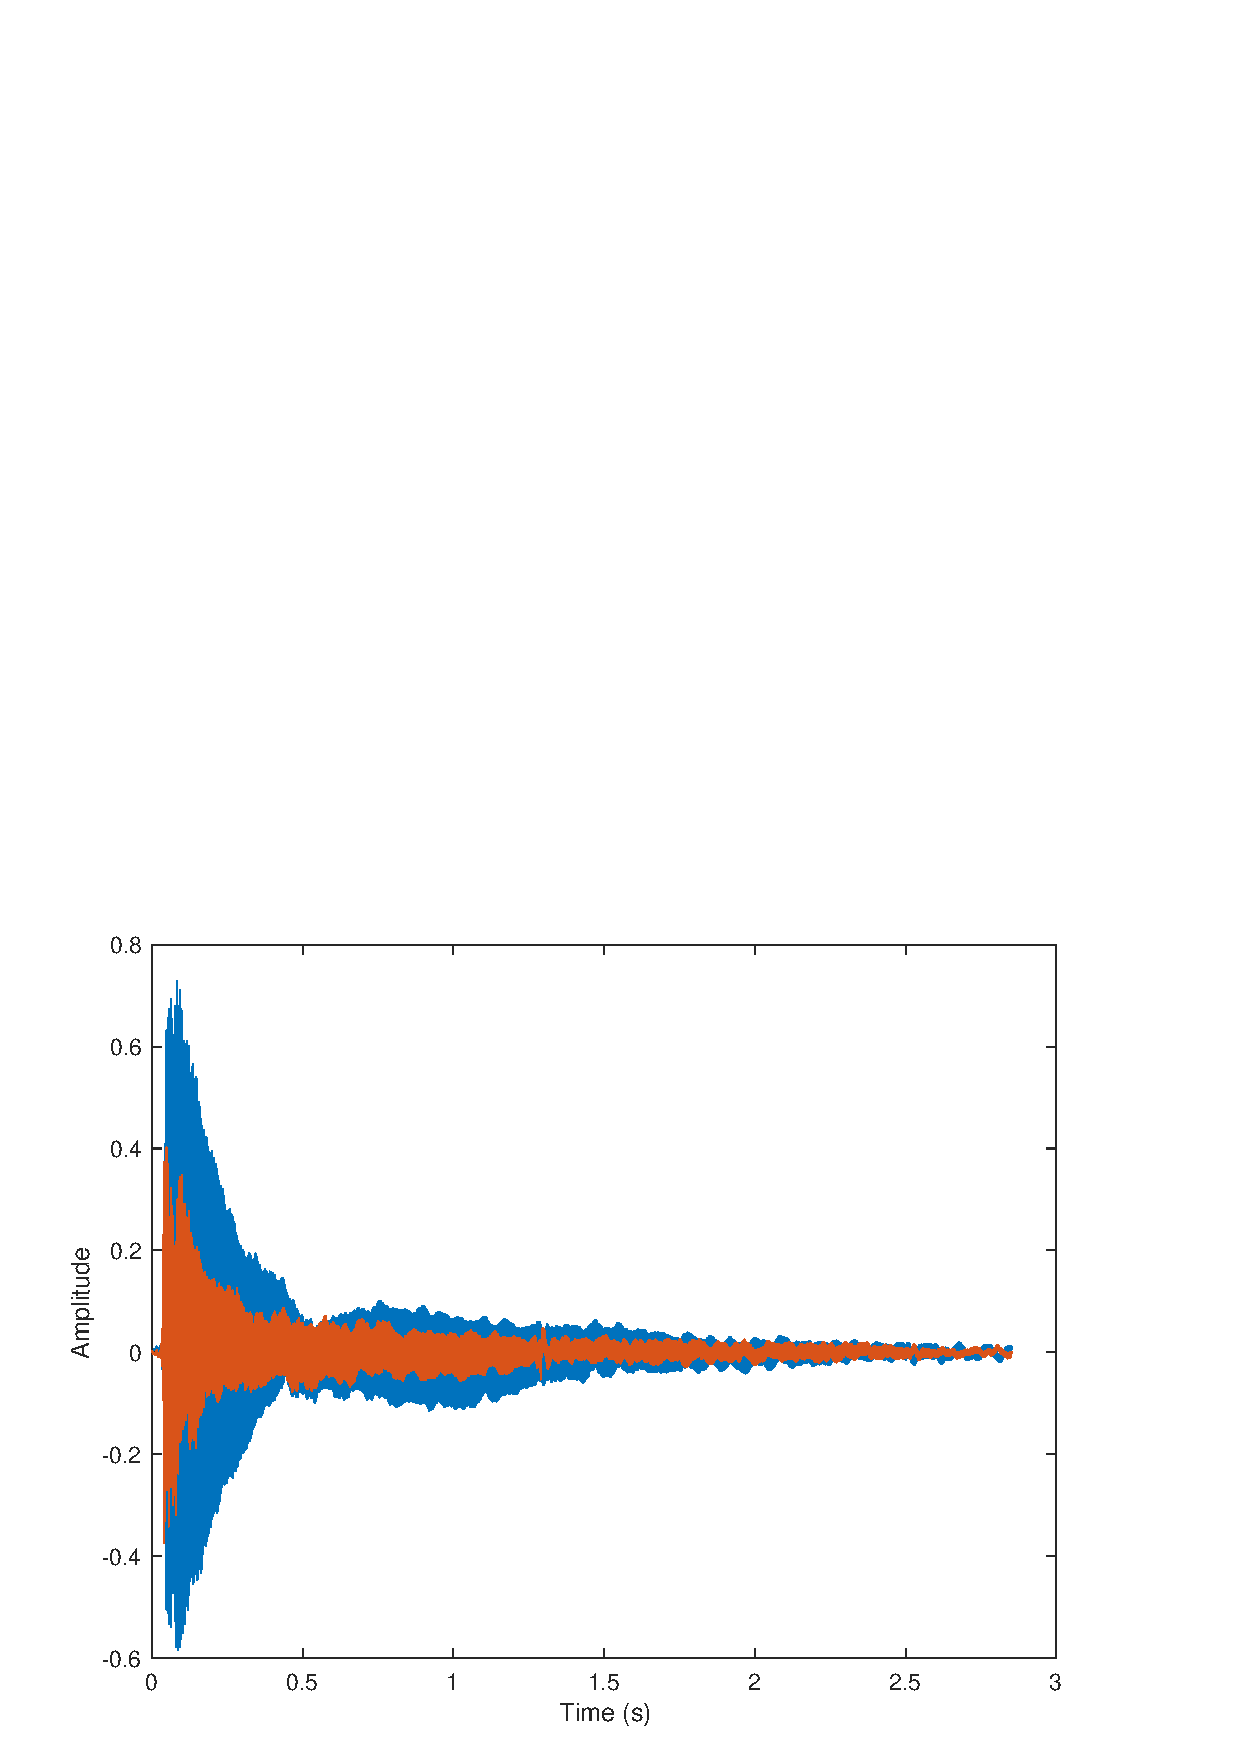
\includegraphics[width = 0.45\textwidth]{signal_before_mean.png}
}
\subfigure[Exemple de signal moyenné]{
\label{Fig.sub.2}
\includegraphics[width = 0.45\textwidth]{signal_after_mean.png}
}
\caption{Exemple de signal}
\label{Fig.main}
\end{figure}
